%% sections/methodology.tex

\section{Methodology}
\label{sec:methodology}

\subsection{Architecture Overview}

RADAR is a multimodal binary classifier that combines deep contextual representations with handcrafted stylometric features. As shown in Figure~\ref{fig:architecture}, the model consists of four components: (1) the \textbf{Adversarially Robust Semantic Encoder} (\arse), (2) the \textbf{Statistical Linguistic Profile Extractor} (\slpe), (3) a \textbf{Cross-Attention Fusion} layer, and (4) the \textbf{Unified AI Content Classifier} (\uacc). The design is deliberately modular: each component addresses a distinct aspect of the detection problem, and together they cover a broad, complementary feature space.

\begin{figure}[htbp]
  \centering
  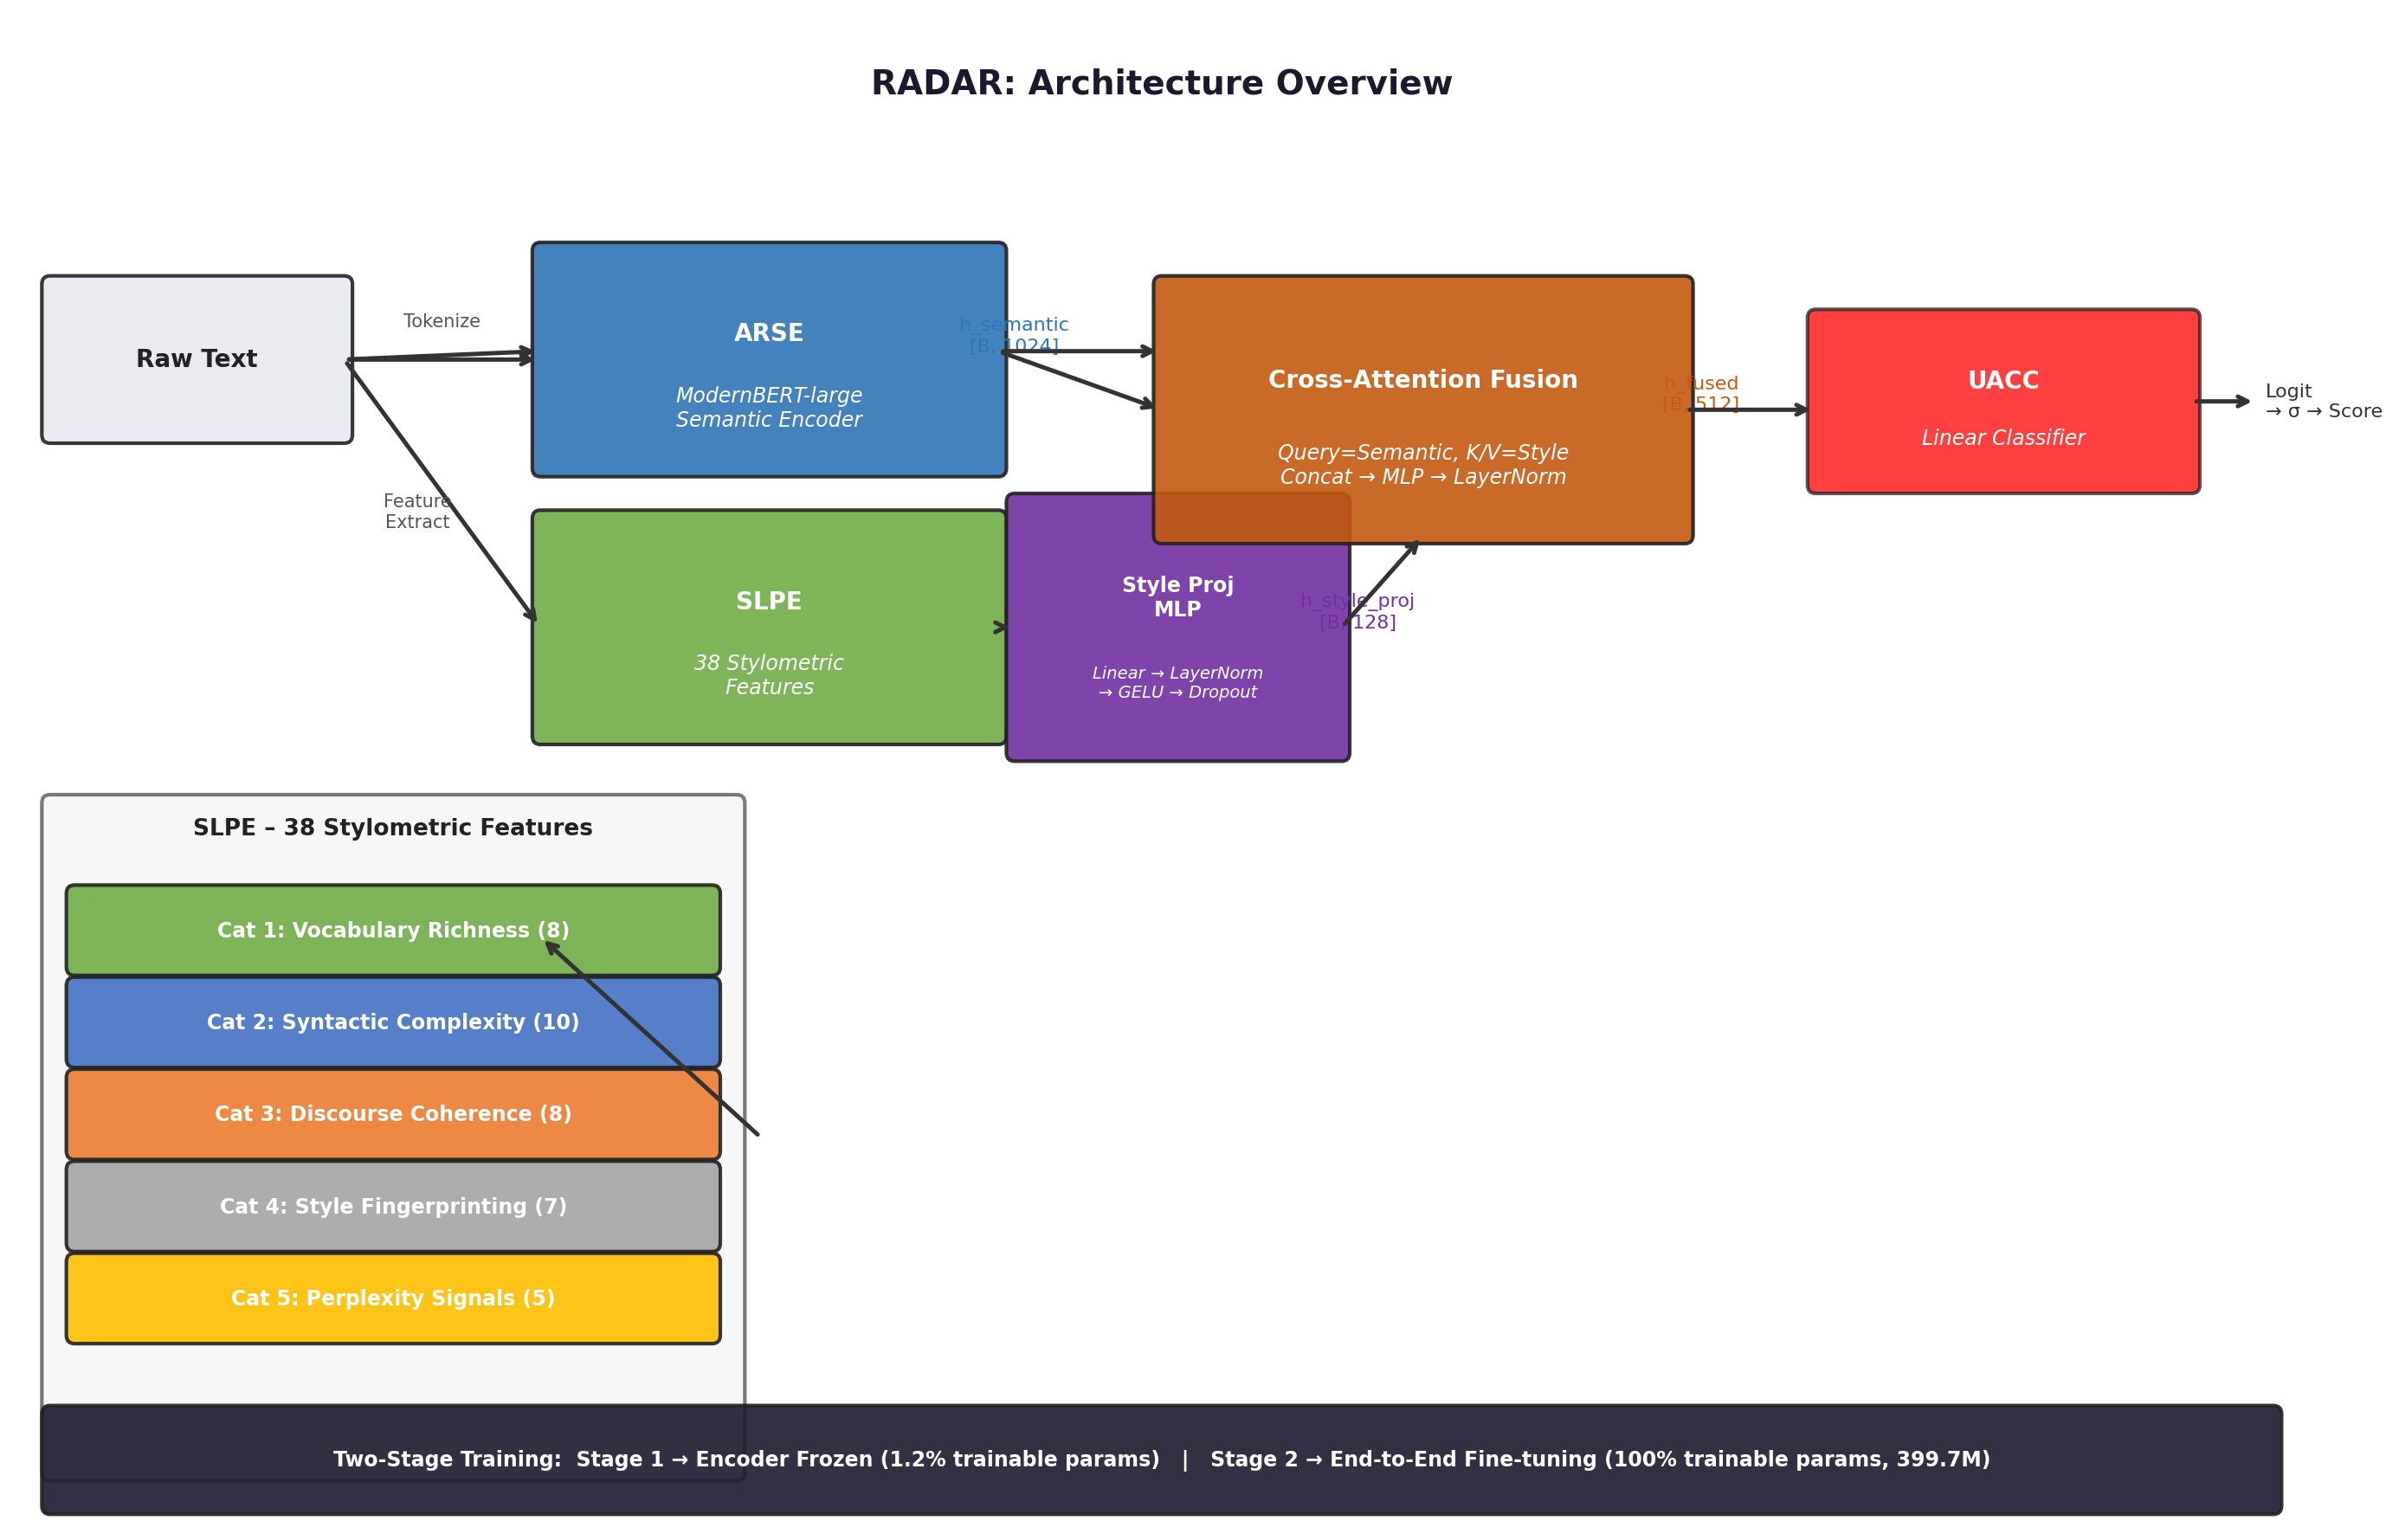
\includegraphics[width=\linewidth]{images/radar_architecture.png}
  \caption{RADAR architecture. The input text is processed in parallel by the semantic
           encoder (ARSE) and the stylometric feature extractor (SLPE). Their outputs
           are fused through a cross-attention mechanism and passed to the classifier.}
  \label{fig:architecture}
\end{figure}

\subsection{ARSE: Semantic Encoder}

The semantic stream is handled by ModernBERT-large~\cite{modernbert:2024}, a recently introduced bidirectional encoder that significantly improves on BERT~\cite{devlin:2019} and RoBERTa~\cite{liu:2019} along several dimensions: it supports sequences of up to 8,192 tokens via a rotary position embedding (RoPE) scheme, uses alternating global and local attention for efficiency, and was pre-trained on 2 trillion tokens from a wide range of domains and programming languages.

Given an input text, ARSE tokenizes it and runs it through the full ModernBERT-large transformer stack. We extract the hidden state of the special \texttt{[CLS]} token from the final layer as the sentence-level semantic representation:
\begin{equation}
  \mathbf{h}_{\text{sem}} = \text{ModernBERT}(\mathbf{x})_{[0,:]} \in \mathbb{R}^{1024}.
\end{equation}
This representation captures global semantic content, topic modelling, and grammatical structure in a dense, 1024-dimensional vector. ModernBERT-large contributes approximately 395 million parameters to RADAR.

\subsection{SLPE: Stylometric Feature Extractor}

The stylometric stream is computed by a fully rule-based, lightweight extractor that operates on the raw tokenised text without any neural components. \slpe produces a 38-dimensional feature vector $\mathbf{f} \in [0,1]^{38}$ organised into five categories:

\subsubsection{Category 1 -- Vocabulary Richness (8 features)}
These features quantify the lexical diversity of the text:
\begin{itemize}
  \item \textit{Type-Token Ratio (TTR)}: unique words divided by total words.
  \item \textit{Hapax Legomena ratio}: proportion of words occurring exactly once.
  \item \textit{Brunet's $W$}: $N^{V^{-0.172}}$, a size-corrected vocabulary measure.
  \item \textit{Honore's $R$}~\cite{honore:1979}: $100 \cdot \log N / (1 - h_1/V)$, where $h_1$ is the hapax count and $V$ is the vocabulary size; normalised and capped to $[0,1]$.
  \item \textit{MATTR}: Moving-Average TTR with a 100-word window, which compensates for text-length effects.
  \item \textit{Vocabulary richness slope}: linear trend of TTR across consecutive windows, capturing how quickly new words are introduced.
  \item \textit{Rare word frequency}: identical to hapax ratio, used as an independent feature.
  \item \textit{Function word density}: proportion of closed-class (grammatical) words.
\end{itemize}

LLMs tend to exhibit more uniform vocabulary reuse and flatter TTR slopes than humans; these features directly capture this difference.

\subsubsection{Category 2 -- Syntactic Complexity (10 features)}
Syntactic features quantify the structural organisation of sentences:
\begin{itemize}
  \item Average sentence length and sentence-length variance (normalised).
  \item Clause density: commas per sentence as a subordinate clause proxy.
  \item Subordination ratio: subordinating conjunctions per sentence.
  \item Passive voice frequency: heuristic based on auxiliary + past-participle patterns.
  \item Noun phrase proxy: mid-sentence capitalised tokens (proper nouns and titles).
  \item Verb density: auxiliary and inflected verb forms per word.
  \item Coordination frequency: coordinating conjunctions per word.
  \item Mean relative word position: average within-sentence position (constant 0.5 for human-like variation).
  \item Sentence-length skewness: third standardised moment of sentence-length distribution.
\end{itemize}

\subsubsection{Category 3 -- Discourse Coherence (8 features)}
These features measure how ideas flow across sentences and paragraphs:
\begin{itemize}
  \item \textit{Lexical cohesion}: mean Jaccard similarity between adjacent sentence vocabularies.
  \item \textit{Pronoun density}: pronoun frequency as a coreference proxy.
  \item \textit{Transition word frequency}: discourse markers per sentence.
  \item \textit{Paragraph coherence}: mean cosine similarity of adjacent paragraph term-frequency vectors.
  \item \textit{Topic consistency}: vocabulary overlap between first and last paragraph.
  \item \textit{Information flow variance}: variance in the rate at which new words are introduced.
  \item \textit{Semantic repetition}: proportion of repeated word tokens.
  \item \textit{Connective marker diversity}: unique transition words over total transition words.
\end{itemize}

LLM-generated texts tend to have higher inter-sentence lexical cohesion and more formulaic transition word usage than human texts.

\subsubsection{Category 4 -- Style Fingerprinting (7 features)}
Surface-level style markers:
\begin{itemize}
  \item Punctuation density, capitalisation ratio, digit frequency, quote-character frequency.
  \item Parenthetical frequency per sentence.
  \item Paragraph-length variance.
  \item List-structure frequency (lines starting with bullet or numbered markers).
\end{itemize}

\subsubsection{Category 5 -- Perplexity Signals (5 features)}
These features approximate language-model perplexity using corpus statistics only, without any external model:
\begin{itemize}
  \item \textit{Forward word entropy}: mean negative log-probability of each word under the text's own unigram distribution.
  \item \textit{Backward entropy}: same, computed in reverse order.
  \item \textit{Entropy ratio}: forward/backward entropy ratio, capturing directional information asymmetry.
  \item \textit{Burstiness}: variance of per-word surprisal values; high burstiness is characteristic of human writing (alternating common and rare words).
  \item \textit{Mean surprisal}: average information content per word.
\end{itemize}

All 38 features are normalised to $[0,1]$, and any NaN or infinite value is replaced with zero.

The projected stylometric representation is computed by a small MLP:
\begin{equation}
  \mathbf{h}_{\text{style}} = \text{GELU}(\text{LayerNorm}(\mathbf{W}_s \mathbf{f} + \mathbf{b}_s)) \in \mathbb{R}^{128},
\end{equation}
where dropout regularises the projection during training.

\subsection{Cross-Attention Fusion}

The fusion layer combines $\mathbf{h}_{\text{sem}} \in \mathbb{R}^{1024}$ and $\mathbf{h}_{\text{style}} \in \mathbb{R}^{128}$ through a single-head-to-head cross-attention step followed by a projection MLP:

\begin{enumerate}
  \item Project the style vector to the semantic dimension: $\tilde{\mathbf{h}}_s = \mathbf{W}_{s\to q}\, \mathbf{h}_{\text{style}} \in \mathbb{R}^{1024}$.
  \item Compute cross-attention with $\mathbf{h}_{\text{sem}}$ as query and $\tilde{\mathbf{h}}_s$ as key and value (8 heads, head dimension 128):
    \begin{equation}
      \mathbf{a} = \text{MultiHeadAttn}(\mathbf{h}_{\text{sem}}, \tilde{\mathbf{h}}_s, \tilde{\mathbf{h}}_s) \in \mathbb{R}^{1024}.
    \end{equation}
  \item Apply a residual connection and layer normalisation:
    \begin{equation}
      \hat{\mathbf{a}} = \text{LayerNorm}(\mathbf{a} + \mathbf{h}_{\text{sem}}).
    \end{equation}
  \item Concatenate with the original style projection and project to the fusion dimension:
    \begin{equation}
      \mathbf{h}_{\text{fused}} = \text{GELU}(\text{LayerNorm}([\hat{\mathbf{a}},\, \mathbf{h}_{\text{style}}]\,\mathbf{W}_f + \mathbf{b}_f)) \in \mathbb{R}^{512},
    \end{equation}
    where $[\cdot,\cdot]$ denotes concatenation.
\end{enumerate}

This design allows the semantic representation to selectively attend to the stylometric evidence—focusing on the style dimensions that are most diagnostic given the current text—before the two streams are concatenated and projected.

\subsection{UACC: Classifier Head}

The final classification head is a single linear layer mapping the 512-dimensional fused representation to a scalar logit:
\begin{equation}
  z = \mathbf{w}^\top \mathbf{h}_{\text{fused}} + b \in \mathbb{R}.
\end{equation}
The probability of AI authorship is $\hat{p} = \sigma(z)$, where $\sigma$ is the sigmoid function. During training, we minimise binary cross-entropy with logits:
\begin{equation}
  \mathcal{L} = -\Bigl[y\,\log\sigma(z) + \omega\,(1-y)\,\log(1-\sigma(z))\Bigr],
\end{equation}
where $\omega$ is a class-rebalancing weight computed from the training set label distribution.

\subsection{Two-Stage Training Strategy}

RADAR is trained in two stages, as illustrated at the bottom of Figure~\ref{fig:architecture}:

\textbf{Stage~1 -- Encoder Freeze.} We freeze the ModernBERT-large encoder and train only the stylometric projector, fusion layer, and classifier. This constitutes 4,929,665 trainable parameters out of 399,711,361 total (1.2\%). The motivation is twofold: (i) it forces the lightweight components to learn from both the fixed semantic representations and the stylometric features without overfitting, and (ii) it produces a stable initialisation for Stage~2 that avoids catastrophic forgetting of pre-trained knowledge.

\textbf{Stage~2 -- End-to-End Fine-tuning.} Starting from the Stage~1 checkpoint, we unfreeze all parameters and train the full model end-to-end at a low learning rate with a cosine schedule. This allows the encoder to adapt its internal representations to the detection objective while retaining the robustness of the Stage~1 solution.

\subsection{Inference}

At inference time, RADAR tokenizes the input text (up to 512 tokens), extracts the 38-dimensional stylometric feature vector, runs both streams through the model, and outputs $\hat{p} \in [0,1]$. Texts with $\hat{p} > 0.5$ are classified as AI-generated, and the raw probability is used as the confidence score for the PAN evaluator. Processing is independent for each text, satisfying the task's requirement of no leakage between test cases.
